\documentclass[a4paper,11pt]{article}

\usepackage[T1]{fontenc}
\usepackage[swedish]{babel} 
\usepackage[utf8]{inputenc}
\usepackage{graphicx}
\usepackage{placeins}
\usepackage[small]{caption}

\usepackage{fancyhdr}
\pagestyle{fancy}

\fancyhead{}
\fancyfoot{}

\fancyhead[L]{Grafer och planäritet}
\fancyhead[R]{Peter Boström -- \emph{pbos@kth.se}}
\fancyfoot[C]{Diskret matematik, SF1631}
\fancyfoot[R] {\thepage}

\title{Grafer och planäritet}
\author{Peter Boström -- \emph{pbos@kth.se}}

\begin{document}
\maketitle
\pagestyle{fancyplain}

\begin{abstract}
Uppsatsen går igenom en rad grundläggande begrepp för grafer för att ge en bakgrund som krävs för att förstå uppsatsen. Bland annat vad de är, bipartita grafer och kompletta grafer.

Sedan diskuteras plana och planära grafer vilket innebär om grafen kan ritas plant eller inte. Kriterier för detta samt Kuratowskis sats presenteras, intuitiva motiveringar för $K_5$ samt $K_{3,3}$:s ickeplanäritet presenteras.

Slutligen som exempel på ett praktiskt användningsområde diskuteras kortfattat hur grafer kan representera kretskort samt hur planäritet påverkar hur de kan tryckas.

\end{abstract}
\clearpage

\section*{Grafer, kompletta grafer och andra begrepp}

En \textbf{graf} är en samling, eller \emph{mängd}, av så kallade \emph{noder} och \emph{kanter} som ansluter mellan två noder. En nod kan ses som en punkt och kant kan ses som ett sträck draget mellan två av dessa noder. En kant bör även ses som en anslutning mellan två noder.

\begin{figure}[!ht]
	\begin{center}
		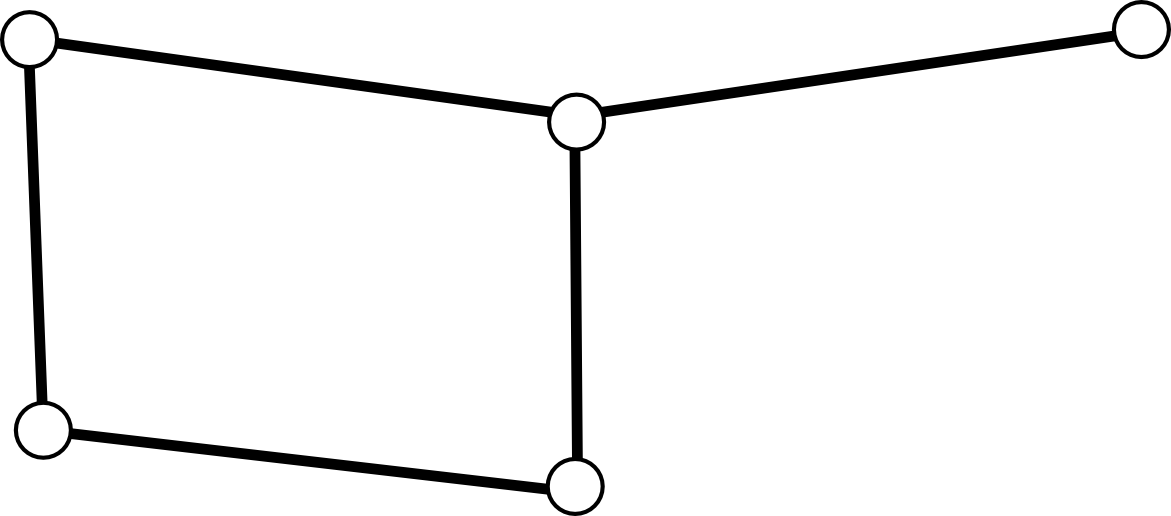
\includegraphics{fig1}
		\caption{En graf med 5 noder och 5 kanter.}
		\label{fig1}
	\end{center}
\end{figure}
\FloatBarrier

En \textbf{bipartit graf} är en graf där grafen kan delas upp i två grupper av noder som inte har några kanter internt mellan sig, men tillåts ha anslutningar mellan noder i de olika grupperna.

\begin{figure}[!ht]
	\begin{center}
		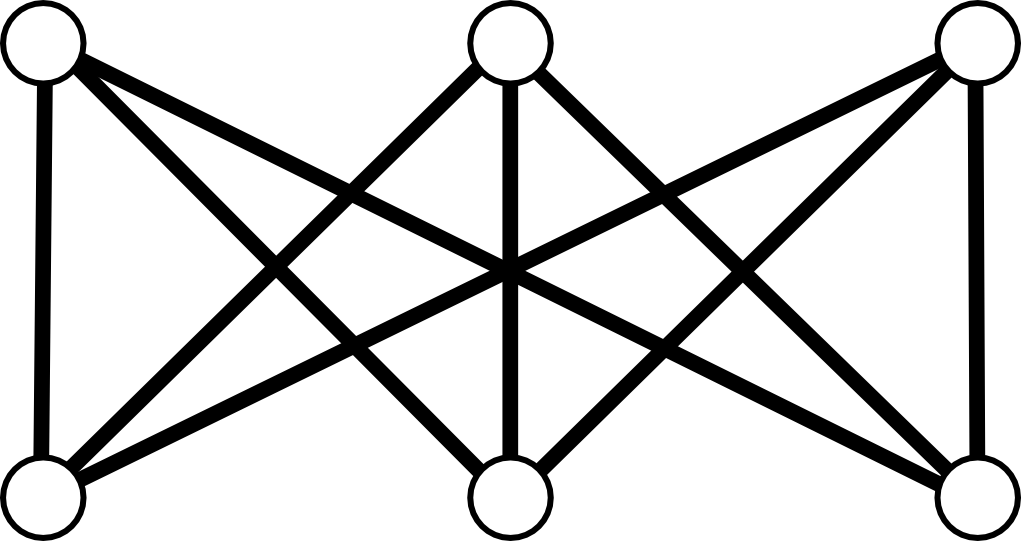
\includegraphics{fig2}
		\caption{Bipartit graf med två grupper om 3 noder vardera.}
		\label{fig2}
	\end{center}
\end{figure}
\FloatBarrier

En \textbf{komplett graf} är en graf där varje nod har en kant som ansluter med varje annan nod. Kompletta grafer tecknas $K_n$ där $n$ står för antalet noder i den kompletta grafen.

\begin{figure}[!ht]
	\begin{center}
		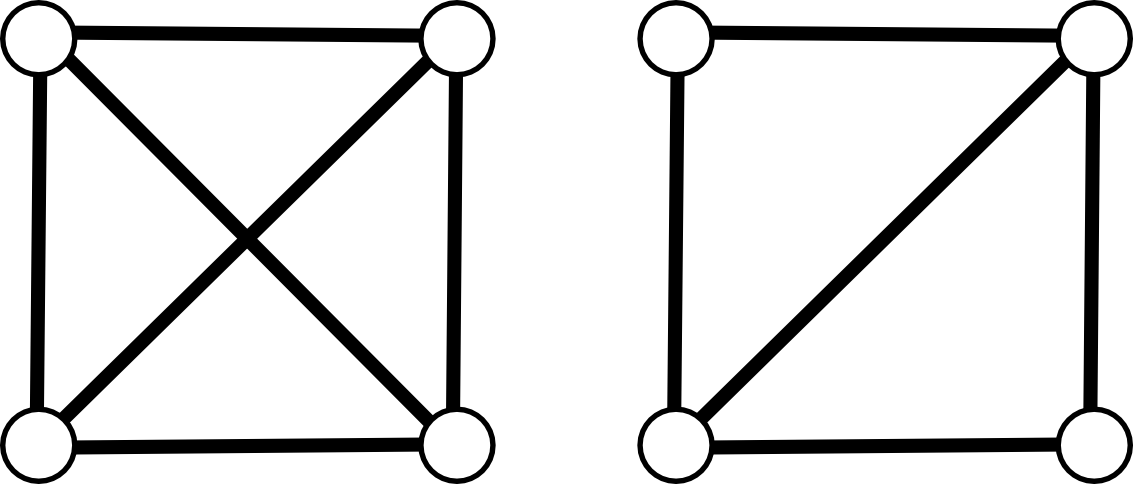
\includegraphics{fig3}
		\caption{Bild på $K_4$ till vänster. Grafen till höger är inte komplett då det saknas en kant mellan två av noderna.}
		\label{fig3}
	\end{center}
\end{figure}
\FloatBarrier

\textbf{Kompletta bipartita grafer} tecknas $K_{n,m}$ och har två grupper av noder med $n$ respektive $m$ stycken noder där varje nod i en grupp ansluter till varje nod i den andra gruppen. Figur \ref{fig2} är ett exempel på en komplett bipartit graf, $K_{3,3}$. Notera att $n$ och $m$ lika gärna kan vara olika tal.

\section*{Grafers planäritet}

En graf är \textbf{plan} om den är tecknad så att inga kanter korsar varandra. Man kan tänka sig att att grafen är plan betyder att den är helt platt.

\begin{figure}[!ht]
	\begin{center}
		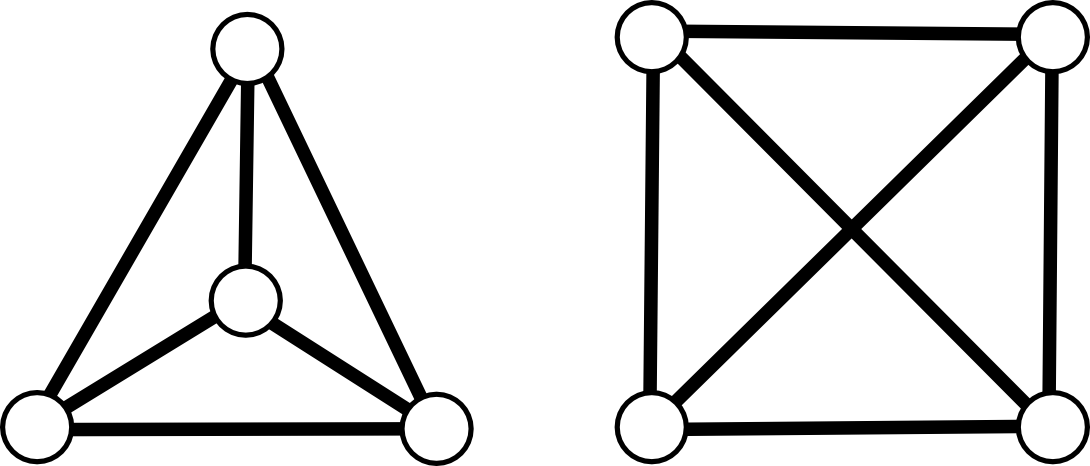
\includegraphics{fig4}
		\caption{Båda grafer bildar den kompletta grafen $K_4$. Den vänstra grafen är plan medan den högra inte är det då (minst) två kanter korsar varandra.}
		\label{fig4}
	\end{center}
\end{figure}
\FloatBarrier

En \textbf{planär graf} är en graf som \emph{kan} ritas plant, men inte nödvändigtvis är plant ritad. I exemplet ovan, figur \ref{fig4}, är endast den vänstra grafen plan medan båda grafer är planära.

Grafers planäritet har viktiga verkliga användningsområden. Ett vanligt exempel är under konstruktion av kretskort då om ledningarna som dras korsar varandra blir det kortslutning. Till detta användningsområde återkommer vi i slutet av uppsatsen.

Bildar dessa en planär graf går kretskortet att konstruera på enbart ett lager.

\section*{Icke-planära grafer}

Grafer som inte går att rita plant kallas för \textbf{icke-planära grafer}. Ett exempel på en icke-planär graf är kompletta grafen med 5 noder, $K_5$.

\begin{figure}[!ht]
	\begin{center}
		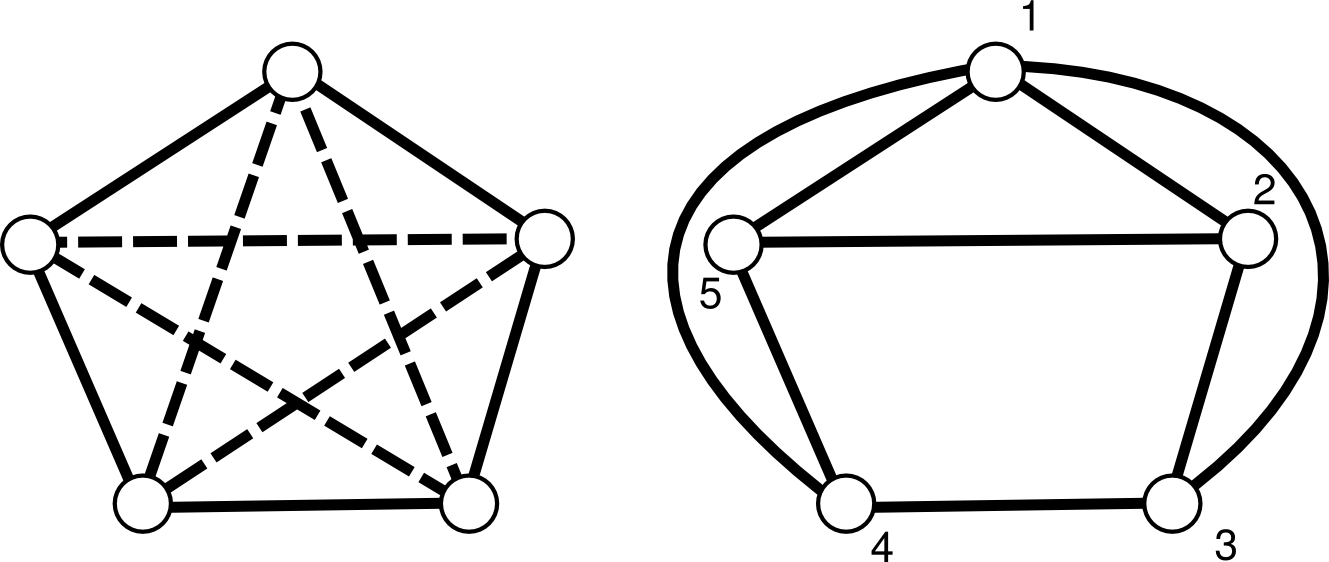
\includegraphics{fig5}
		\caption{Kompletta grafen $K_5$, till vänster, samt figur för att illustrera varför grafen inte går att rita plant.}
		\label{fig5}
	\end{center}
\end{figure}
\FloatBarrier

Bilden till vänster är hur vi $K_5$ vanligt ritas.
Vi förstår att alla noder måste sitta ihop med alla, så först kopplar vi ihop noderna till en pentagon.
För alla ytterligare anslutningar gäller det att kanterna, för att den ska ritas planärt, måste ligga antingen helt innanför eller utanför pentagonen, då de annars kommer att korsa existerande kanter.

Om vi antar att t.ex. nod $5$ och nod $2$, se figur \ref{fig5}, är sammankopplade innanför polygonen kommer det att avgränsa nod $1$ från nod $4$ och $5$ inuti hexagonen.
Därför måste kanterna mellan nod $1$ och nod $4$ samt nod $1$ och nod $5$ ritas utanför polygonen.
Kanten som dras mellan $3$ och $5$ hade kunnat dras till vänster om resten av grafen, men båda dessa teckningar medför att ingen av de två kanter som ska finnas mellan nod $2$ och nod $4$ samt nod $5$ och nod $3$ kan ritas utanför pentagonen utan att korsa någon av dessa kanter.
Kvar har vi då att kanterna mellan nod $2$ och nod $4$ måste ritas innanför pentagonen, vilket omöjligt kan göras utan att dessa korsar varandra.

Alltså är $K_5$ inte planär. Då $K_4$ som tidigare nämnts är planär är $K_5$ den minsta kompletta grafen som samtidigt inte är planär.

En annan graf som inte går att rita plant är $K_{3,3}$.

\begin{figure}[!ht]
	\begin{center}
		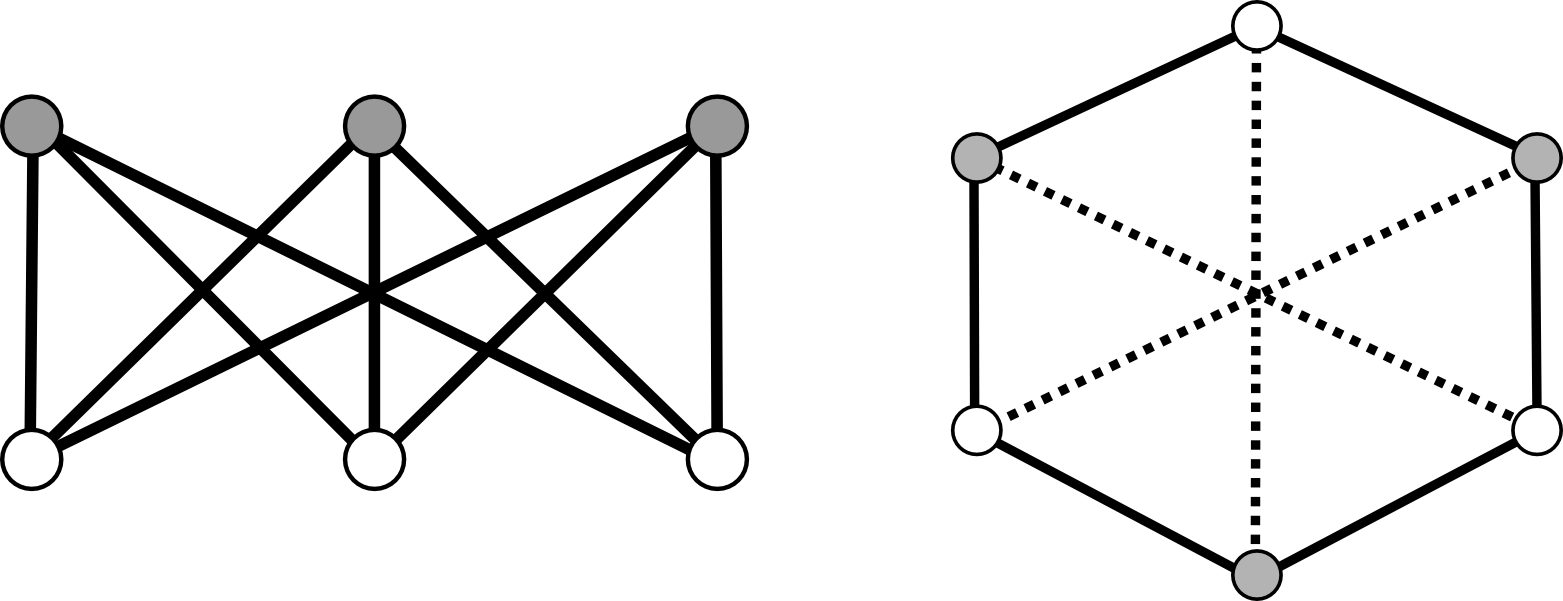
\includegraphics{fig6}
		\caption{Kompletta bipartita grafen $K_{3,3}$. Till höger är den ritad som en hexagon liknande figuren ovan.}
		\label{fig6}
	\end{center}
\end{figure}
\FloatBarrier

Att $K_{3,3}$ är icke-planär förklaras på liknande sätt. I denna hexagon kan varken två extra kanter ritas plant inuti eller utanför hexagonen. Eftersom tre totalt ska ritas, och varken två av dem kan placeras inuti eller utanför, så är $K_{3,3}$ icke-planär.

$K_{2,3}$ däremot är planär, så $K_{3,3}$ är då den minsta icke-planära kompletta bipartita grafen.

\begin{figure}[!ht]
	\begin{center}
		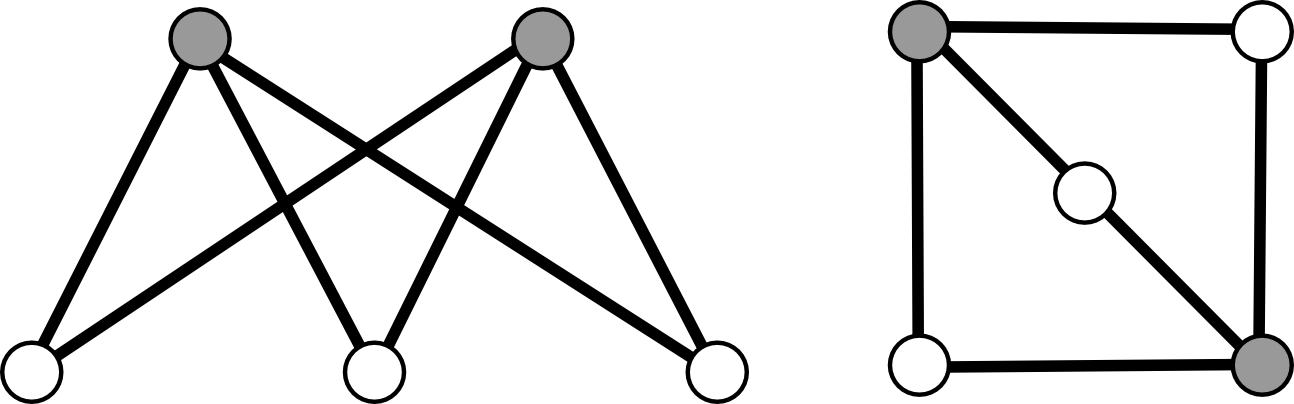
\includegraphics{fig7}
		\caption{Planära kompletta bipartita grafen $K_{2,3}$, till vänster tecknad som vanligt och till höger tecknad plant.}
		\label{fig7}
	\end{center}
\end{figure}
\FloatBarrier

\section*{Homomorfa grafer och större icke-planära grafer}

En homomorfi mellan två innebär att den ena grafen på ett eller annat sätt innehar samma egenskaper som den andra. Dvs. att de på ett eller annat sätt är identiska. Det kan handla om att den innehåller triviala tillägg som inte påverkar dess egenskaper. Notera att varje graf är homomorf med sig själv.

\begin{figure}[!ht]
	\begin{center}
		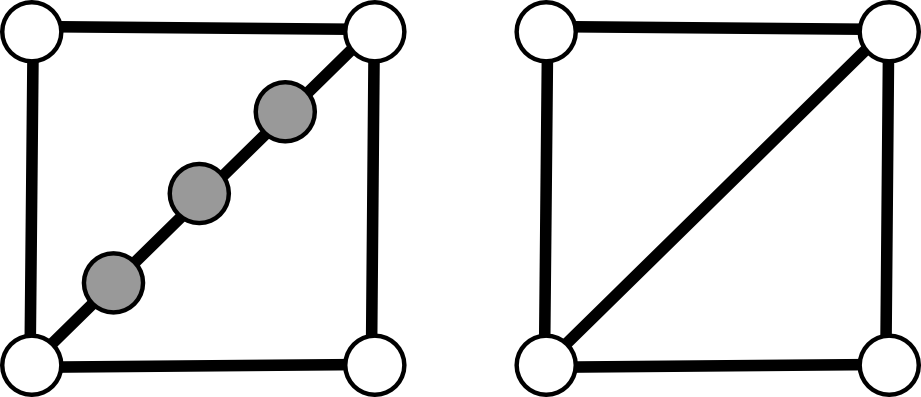
\includegraphics{fig8}
		\caption{Exempel på där vänstergrafen är homomorfa med den högra. I vårt fall är det uppenbart att extra noder på en kant inte påverkar dess planäritet då en kant redan kan böjas hur som helst när den ritas ut.}
		\label{fig8}
	\end{center}
\end{figure}
\FloatBarrier

Det har visat sig att ingen planär graf har en delgraf som är homomorf med $K_{5}$ eller $K_{3,3}$.
Detta påstående kallas för Kuratowskis teorem och är mycket viktigt för att kunna bestämma om grafer är planära eller inte. 
Beviset däremot är komplicerat och lämnas att eventuellt undersökas av den intresserade läsaren.

Notera att varje komplett graf med fler än $5$ noder innehåller $K_5$ som delgraf. Notera även att varje kompletta bipartita graf där båda grupper av noder är om 3 eller fler noder innehåller $K_{3,3}$ som delgraf.

Ett annat exempel på en grafhomomorfi är att planära delgrafer går att dra ihop till en nod utan att skapa ytterligare korsningar, då de kan ritas oändligt små. Delgrafen kan inte dras ihop på det här sättet om den innehåller fler än en anslutning till en annan nod.

\begin{figure}[!ht]
	\begin{center}
		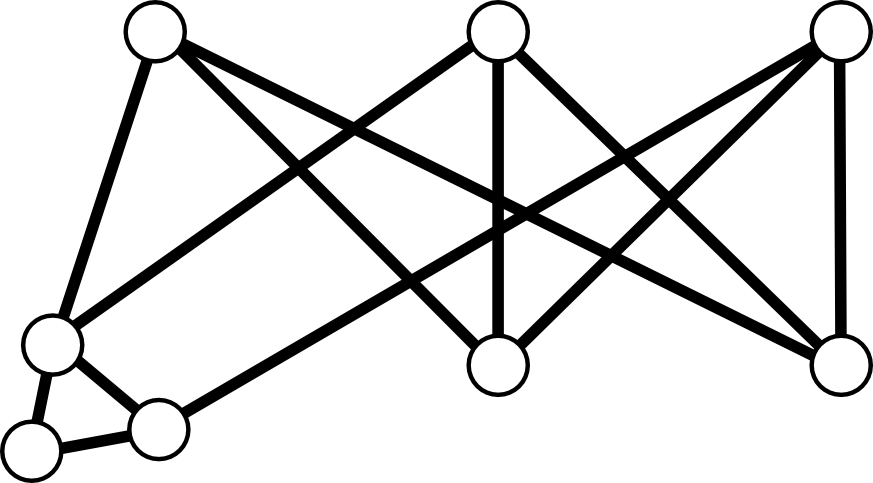
\includegraphics{fig9}
		\caption{Icke-planär graf som varken har $K_5$ eller $K_{3,3}$ som direkt delgraf.}
		\label{fig9}
	\end{center}
\end{figure}
\FloatBarrier

Exemplet ovan illustrerar hur homomorfi är viktigt för att kunna avgöra om en graf är planär eller inte. Dras den planära delgrafen längst ner till vänster ihop till en nod så blir grafen den icke-planära kompletta bipartita grafen $K_{3,3}$.

\section*{Planära grafer och kretskortskonstruktion}

Ett vanligt exempel på praktiskt område där planäritet är viktigt är kretskortkonstruktion, som tidigare nämnt. På ett kretskort konstrueras ledningar på samma lager så att ifall två ledningar korsar varandra så blir det kortslutning. Det går även att konstruera kretskort med flera lager så att det går att tillåta att två ledningar korsar varandra.

Om vi förenklat antar att en ledning kan anslutas var som helst på en komponent så blir varje komponent en nod och en ledning mellan två komponenter en kant. En ledning antas enbart ansluta mellan två komponenter, vilket är vanligt. Jordning för ledningarna kan ses som en komponent.

\begin{figure}[!ht]
	\begin{center}
		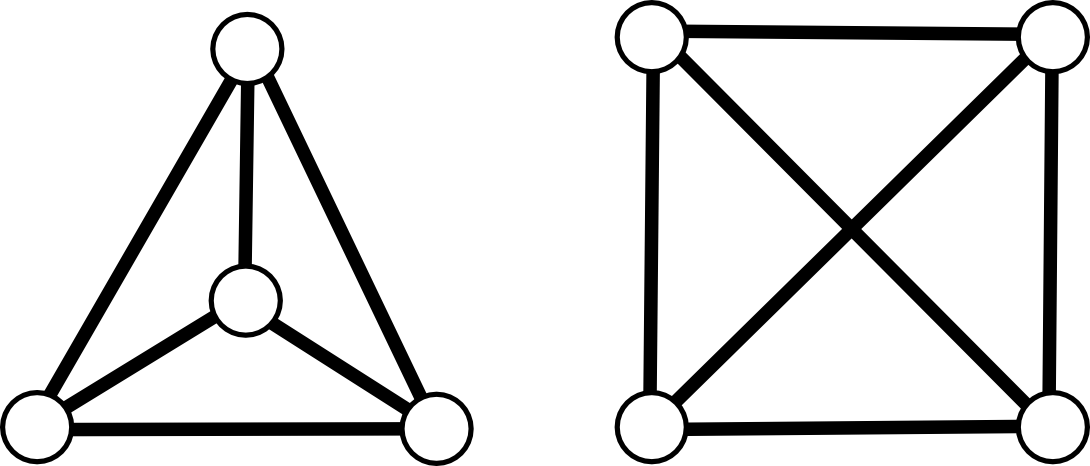
\includegraphics{fig4}
		\caption{En grafisk representation av en kretskortsdesign där fyra komponenter alla ska kopplas till varandra. Till vänster är grafen plant ritad medan grafen till höger är hur man kanske spontant skulle rita grafen.}
		\label{fig4:2}
	\end{center}
\end{figure}
\FloatBarrier

Har vi då en design där 4 komponenter behöver kopplas till varandra så kan vi, som vi ser till vänster, trycka upp detta kretskort så att inga ledningar korsar varandra. Därför går kretskortet att trycka på enbart ett lager. Detta förenklar tillverkningsprocessen och gör även kretskortet billigare att tillverka.

Är det däremot en ickeplanär design så kommer den inte gå att trycka på ett lager.

\begin{figure}[!ht]
	\begin{center}
		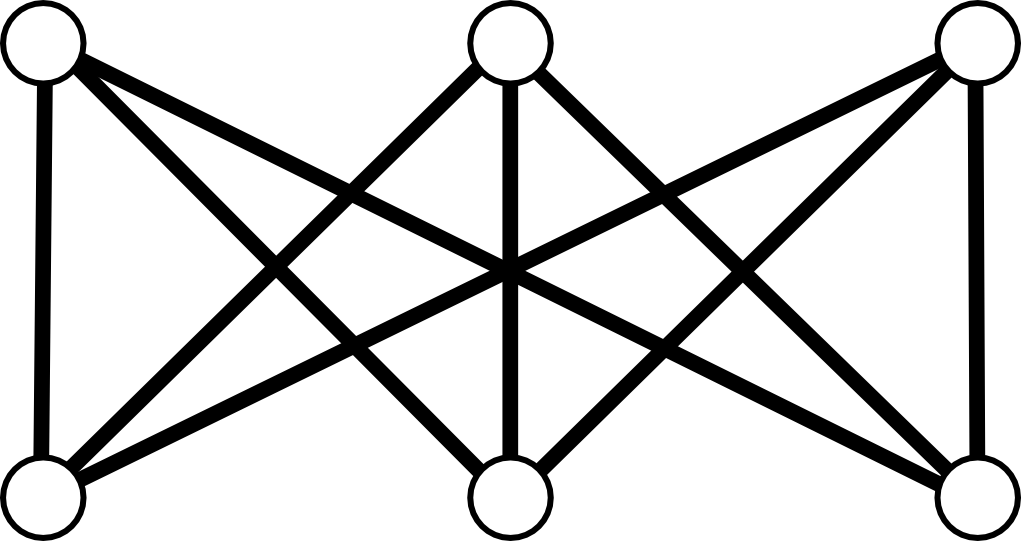
\includegraphics{fig2}
		\caption{En kretskortsdesign där två grupper om tre komponenter där varje komponent behöver kopplas till alla andra i den andra gruppen. Detta bildar den icke-planära kompletta bipartita grafen $K_{3,3}$.}
		\label{fig2:2}
	\end{center}
\end{figure}
\FloatBarrier

Överstående design går inte att rita plant och därför inte att tillverka på ett lager utan att två ledningar korsar varandra. För att trycka denna design krävs då ett kretskort med två lager vilket då är mer komplicerat. Har man inte råd att trycka det här kortet på flera lager så är det viktigt att upptäcka tidigt i designprocessen för att försöka arbeta fram alternativa lösningar för att förenkla kortets design.

\section*{Diskussion}

Att avgöra om en graf är planär eller inte landar i att avgöra om en graf innehåller en delgraf som är homomorf med, dvs. på ett eller annat sett identisk med, $K_5$ eller $K_{3,3}$. Notera att det inte betyder att det är enkelt att avgöra om en graf är planär eller inte, då att finna om en graf innehåller en graf som är homomorf med en annan graf är komplicerat.

Det som är intressant är att \emph{ifall} man finner en delgraf i en graf som är homomorf med någon av dessa två grafer så har man lyckats avgöra att den inte är planär. För att istället bevisa att den är planär är det enklaste beviset, både för att presentera samt för att övertyga, en plan ritning av grafen.

Det är intressant att finna att abstrakta grafer liksom andra matematiska problem har praktiska användningsområden.

Slutligen bör det nämnas att detta inte är allt som finns att säga om planära grafer. Det finns även andra kriterier för att grafer ska vara planära. Dessa lämnas till läsaren att upptäcka. Referensmaterialet till uppsatsen går även mer på djupet och tar upp relaterade koncept, som t.ex. minsta antalet korsningar samt om grafen kan ritas plant på annat än platta ytor, så som en ring med ett, eller flera hål.

\begin{thebibliography}{9}

\bibitem{dongs}
    \emph{Planäritet och Kuratowskis sats}.
      Matematiska Institutionen, KTH. Material utgivet i samband med kurs SF1631,
	  2005.

	  \end{thebibliography}

\end{document}

